\chapter{Resonant Charge Transfer Two Dimensions}
\label{chap:RRP2}

\section{Theory}

% \begin{equation}
% \begin{split}
%   & \Phi_g = \frac{1}{\sqrt{2}}\left(\Phi_a(\vec{r} - \frac{\vec{R}}{2}) + \Phi_b(\vec{r} + \frac{\vec{R}}{2})\right) \\
%   & \Phi_u = \frac{1}{\sqrt{2}}\left(\Phi_a(\vec{r} - \frac{\vec{R}}{2}) - \Phi_b(\vec{r} + \frac{\vec{R}}{2})\right)
% \end{split}
% \end{equation}

% So we now apply the scattering analysis for 2D, from the previous chapter, and assume that $ F_g(r) $ at asymptotic distances obeys the 2D conditions:
% \begin{equation}
%   F_g(R) \underset{R \rightarrow +\infty}{\sim} e^{ik\ x} + f_g(\theta)\frac{e^{ik\ x}}{\sqrt{R}}
% \end{equation}
% Now we use the 2D scattering amplitude from the previous chapter:
% \begin{equation}\label{fgampl}
%   f_g(\theta) = \sqrt{\frac{2}{\pi}}\sum_{m=0}^{\infty}{\epsilon_m \cos(m\theta)e^{i\delta_m^g}\sin\delta_m}
% \end{equation}
% As the $ f(\theta) $ is not directly observable, in 2D we look for the scattering cross section. And we get for the scattering cross section, in 2D:
% \begin{equation}
% \begin{split}
%   & \theta_g = \int_{0}^{2\pi}{d\theta f_g(\theta)} = \frac{2}{\pi}\sum_{m,m'}\int_{0}^{2\pi}{\epsilon_m\epsilon_m' \cos(m\theta)\cos(m'\theta)e^{i\delta_{m}^g}e^{i\delta_{m'}^g}\sin\delta_m^g\delta_{m'}^g} = \\
%   & = \frac{2}{\pi}\sum_{m}{\epsilon_m\sin^2\delta_m^g}
% \end{split}
% \end{equation}

% The same discussion applies for the ungerade solution so we :
% \begin{equation}
%   \theta_u = \frac{2}{\pi}\sum_{m}{\epsilon_m\sin^2\delta_m^u}
% \end{equation}

% In our case we are not interested in the elastic scattering of the gerade and ungerade states,as they form the linear combination of the asymptotic orbitals for the atom A and B, respectively.

% Instead we seek the asymptotic form for the difference
% \begin{equation}
%   \frac{1}{2}\left(F_g(R) - F_u(R)\right) \sim \frac{\left|f_g(\theta) - f_u(\theta)\right|}{4\pi}
% \end{equation}
% Using expression \eqref{fgampl} we get:
% \begin{equation}
% \begin{split}
%   & \sigma = \frac{1}{4}\int_{0}^{2\pi}d\theta\frac{\left|f_g(\theta) - f_u(\theta)\right|^2}{4\pi} \Rightarrow \\
%   & \sigma = \frac{1}{k}\sum_{m}\epsilon_m\sin^2(\delta_u-\delta_g)
% \end{split}
% \end{equation}

% The main approaches to solving these class of problems is to expand the wave function in the partial waves basis and use Born approximation.

% \subsection{Using Partial Waves}

% Using partial waves  we expand the incoming wave in the basis of spherical harmonics, and in the case of azimuthal symmetry to the basis of Legendre polynomials. This in effect mean that we decompose each wave into its constituent angular momentum components and solving using boundary conditions.

% Born approximation \cite{GQuantum} treats a scattering potential as a perturbation to the incoming wave. In this case many partial waves contribute to scattering, so it is preferable to avoid angular momentum decomposition. The Born approximation is generally applicable either when the energy of the incoming particle(s) is high or when the scattering potential is very weak.

% Again we write the time independent Schroedinger equation in 2D:
% \begin{equation}
%   -\frac{1}{2}\nabla^2\psi + V\psi = E\,\psi
% \end{equation}

% where m is the reduced mass, V is a short-range local potential, E is the relative energy.

% Using polar coordinates, setting $ k^2 = 2mE $ , we have the equation
% \begin{equation}
%   \frac{1}{r}\frac{\partial}{\partial r}\left(r\frac{\partial\psi(r,\theta)}{\partial r}\right) + \frac{1}{r^2}\frac{\partial^2\psi(r,\theta)}{\partial \theta^2} + V(r,\theta) = E \psi(r,\theta)
% \end{equation}

% We expand the incoming wave in the partial wave basis as:
% \begin{equation}
%     e^{ikx} = e^{ikr\cos\theta} = \sum_{m=0}^{\infty}{\epsilon_m \cos(m\theta)J_m(kr)}
% \end{equation}
% where $\epsilon_m = 2 $ for $ m \ne 0 $ and $\epsilon_0 = 1 $.


% % We define a scattering cross section in 2 dimensions,, analogous to the scattering cross section in 3D, as:
% % \begin{equation}\label{scatterL}
% %   \sigma(\theta) = |\sqrt{\frac{i}{k}}f_m(\theta)|^2
% % \end{equation}

% % The equation \eqref{squatters} represents the number of particles scattered between $ \theta $ and $ \theta + d\theta $ per second per unit incident flux.

\subsection{Long Range Behavior of $E(R)$ }
In the calculation for the phase shifts, or $b_{m}$, we use the accurate $g,u$ potential curves calculated using the method outlined in Chap. \ref{h2plus2DPotential}.\\

However, for large internuclear separations $ R \approx > 13 a_{0} $, that numerical method becomes unstable. Instead, we match those calculated curves with the analytic asymptotic form described
below.
Although the LCAO approximation given above correctly predicts the asymptotic energy
$ E(R) \rightarrow -2  $ as $ R \rightarrow \infty $, it does not accurately predict the long range behavior of $E(R).$ To that end we note that as $ R \rightarrow \infty $,
\begin{equation}
V({\bf r},{\bf R}) + 1/R \rightarrow -\frac{1}{r}-\frac{z}{R^2} + \frac{x^2-2 z^2}{2 R^3} + \dots
\end{equation}
where $z$ is the electronic coordinate along the direction ${\bf R}$, and we ignored terms that contain higher inverse powers of $R$. Thus the Hamiltonian
\begin{equation}
H \approx H_{0} -\frac{z}{R^2} + \frac{x^2-2 z^2}{2 R^3} + \dots
\end{equation}
where $H_{0}$ is the Hamiltonian for the 2D hydrogen atom. Making use of perturbation theory,
\begin{equation}
E(R) \approx E_{0} + E^{(1)}(R) + E^{(2)}(R) + \cdots
\end{equation}
and
\begin{equation}
E^{(1)} = - \frac{\langle \psi_{1s} |z| \psi_{1s} \rangle }{R^2}
+  \frac{\langle \psi_{1s} |(x^2-2 z^2)| \psi_{1s} \rangle }{2 R^3}  =0
\end{equation}
The lowest non-vanishing contribution arises from second-order perturbation theory
\begin{equation}
  \begin{split}
& E^{(2)} = -\frac{C_{4}}{R^4}  \nonumber \\
& C_{4} = \sum_{n} \frac{|\langle \psi_{1s} |z | \psi_{n} \rangle |^{2} }{E_{1s} - E_{n} }
  \end{split}
\end{equation}
The polarization constant $C_{4} =0.082 $ was given in \cite{YangXL}.


\section{Resonant Charge Transfer Cross Sections}

Consider the amplitude given by expression \eqref{FAmpl}
\begin{equation}
F({\bf R},{\bf r}) = \psi_{g}({\bf R}) \phi_{g}({\bf R},{\bf r}) + \psi_{u}({\bf R}) \phi_{u}({\bf R},{\bf r})
\end{equation}
In the limit as $ R \rightarrow \infty$,
\begin{equation}
F \rightarrow \psi_{g}({\bf R}) \frac{1}{\sqrt{2}} (\phi_{a} + \phi_{b} ) +
\psi_{u}({\bf R}) \frac{1}{\sqrt{2}} (\phi_{a} - \phi_{b} )
\end{equation}
where
\begin{equation}
\phi_{a} \equiv \psi_{1s}({\bf r}-{\bf R}/2)
\quad \phi_{b} \equiv \psi_{1s}({\bf r}+{\bf R}/2)
\end{equation}
Now imposing the boundary conditions
\begin{equation}
\psi_{g,u}({\bf R}) \rightarrow
e^{i k R \cos\phi} + f_{g,u}(\phi) \frac{e^{i k R}}{\sqrt{R}}
\end{equation} 
we get
\begin{equation}
F \rightarrow \sqrt{2}e^{i k R \cos\phi}\phi_{a}
+ \frac{1}{\sqrt{2}} (f_{g}(\phi)+f_{u}(\phi))  \phi_{a}  + \frac{1}{\sqrt{2}} (f_{g}(\phi)-f_{u}(\phi))  \phi_{b}
\end{equation} 
Due to the $ H $ nuclei being equal, the charge-transfer probability is governed by the phase difference. 
So the ratio of flux coming into the $\phi_{a}$ channel to that going into the $\phi_{b} $ channel (i.e. resonant charge transfer) is given by
\begin{equation}
\sigma_{RCT}= \frac{1}{4} \, \int_{0}^{2 \pi} |f_{g}(\phi)-f_{u}(\phi) |^2 = \frac{1}{k} \sum_{m} \Bigl |b^{(g)}_{|m|} - b^{(u)}_{|m|} \Bigr |^2
\end{equation}
where $ b^{(g,u)}_{|m|} $ are the elastic
scattering coefficients for the gerade and ungerade potentials, respectively.

We compute them in the Wolfram Mathematica code listed in appendix \ref{AppendixE}.

 In the figure \ref{fig:CTCS} below we show the plot of the charge transfer cross section in a.u. vs energy. We chose  the range of  $ 10 \mu eV $ to $ 1 meV $ which corresponds to temperatures from $ 0.11 K $ to $ 11 K $.

 \begin{figure}[h]
   \centering
   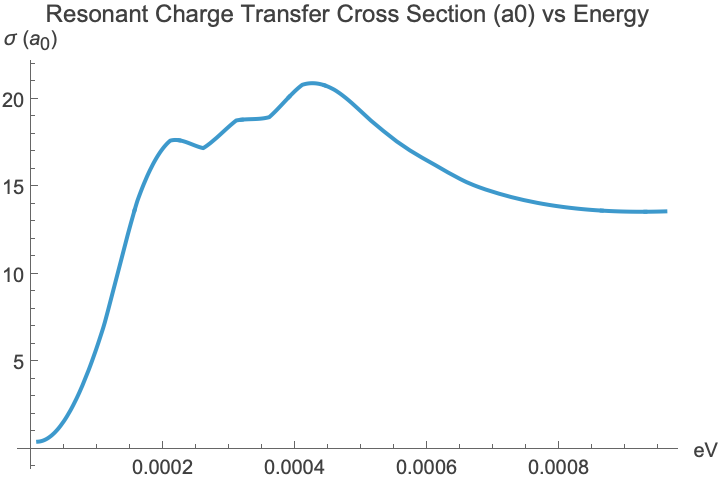
\includegraphics{CTCrossSection1}
   \caption{Charge Transfer Cross Section corresponding to the sum of the first 5 partial waves}
   \label{fig:CTCS}
 \end{figure}

We also calculated the resonant charge transfer cross for each of the first 5 partial waves. The ffigure \ref{fig:CTCS} show the charge transfer cross section for the same energy (temperature) range as a sum of the first 5 partial waves.

\begin{figure*}[htbp]
  \centering
  \begin{subfigure}[t]{0.45\textwidth}
    \centering
    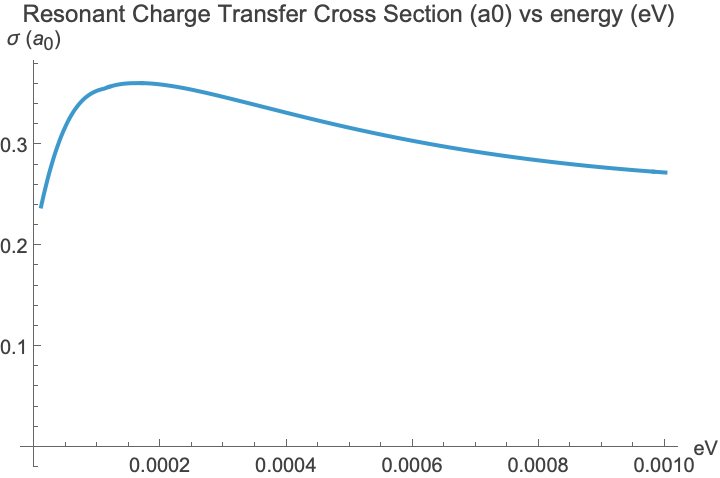
\includegraphics[width=\linewidth]{RCT-1}
    \caption{Resonant Charge Transfer Cross Section, 1st partial wave}
  \end{subfigure}
  \hfill
  \begin{subfigure}[t]{0.45\textwidth}
    \centering
    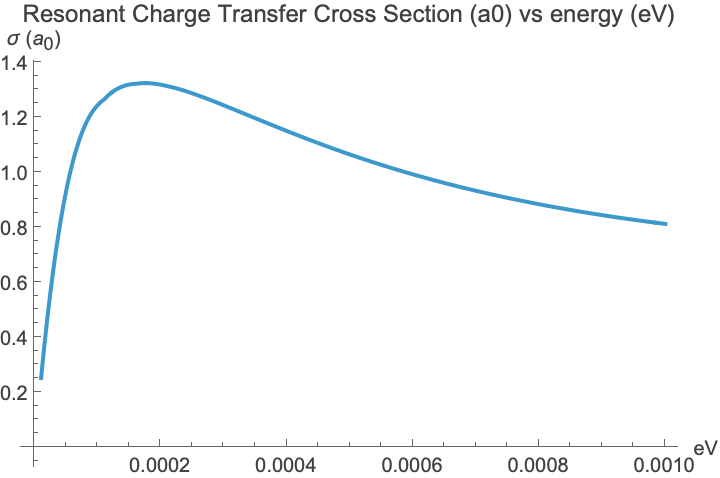
\includegraphics[width=\linewidth]{RCT-2}
    \caption{Resonant Charge Transfer Cross Section, 2nd  partial wave}
  \end{subfigure}
  \begin{subfigure}[t]{0.45\textwidth}
    \centering
    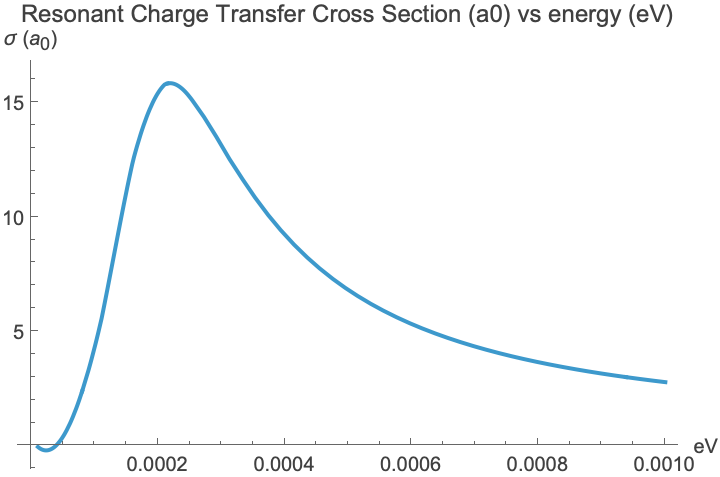
\includegraphics[width=\linewidth]{RCT-3}
    \caption{Resonant Charge Transfer Cross Section, 3rd partial wave}
  \end{subfigure}
  \hfill
  \begin{subfigure}[t]{0.45\textwidth}
    \centering
    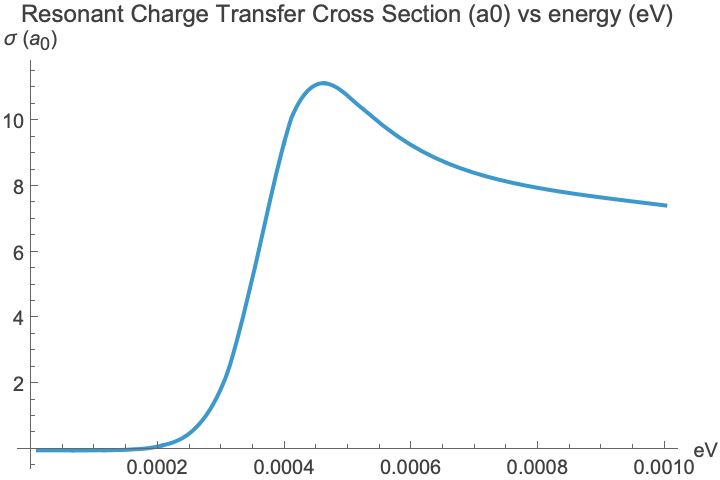
\includegraphics[width=\linewidth]{RCT-4}
    \caption{Resonant Charge Transfer Cross Section, 4th partial wave}
  \end{subfigure}%
  \hfill
  \begin{subfigure}[t]{0.45\textwidth}
    \centering
    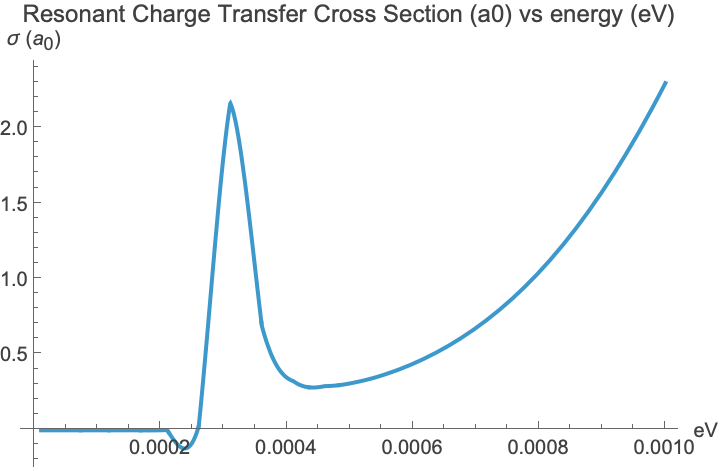
\includegraphics[width=\linewidth]{RCT-5}
    \caption{Resonant Charge Transfer Cross Section, 5th partial wave}
  \end{subfigure}%
  \vfill
  \caption*{Resonant Charge Transfer Cross Section for each of the first 5 partial waves}
\end{figure*}

% \subsection*{Electric Dipole Transition, Einstein A Coefficient: Ground Gerade $\to$ First Ungerade in 2D H$_2^+$}

% Since all the computing machinery was already established we computed the Einstein A Coefficient for the same energy range,
% We used the optical potential method since it does not require an integration over the total spectrum.

% We assume that the system is confined to 2 dimensions while photon are in 3 dimensions, as usual.

% Again it is assumed that the scattering takes place at low energies, so that the system can be described by a wave function $ \Psi(x,t) $ which is itself a solution of a Schrodinger equation $ H\ket{\Psi(t)} = i\hbar\frac{\partial}{\partial t}\ket{\Psi(t)} $ where $ H $ is a Hamiltonian $ H = T + V $ .

% Then we borrow a concept from the optics, where there is a concept of a Complex Refractive Index $ n $. The real part of $ n $ describes how the light is transmitted and the imaginary part describes how the light is absorbed. So it the imaginary part that describes the effect of the scattering. 

% We then express the potential $ V = U + iW $  and the Schrodinger equation becomes $ \left[H + U + iW\right]\ket{\Psi(t)} = i\hbar\frac{\partial}{\partial t}\ket{\Psi(t)} $. 

% From this one gets the scattering cross section:
% \begin{equation}
% \sigma = \frac{k}{E}\int{d^3R\left[-W(R)\right]\left| \psi(R) \right|}
% \end{equation}

% Using the same prolate elliptical coordinates, the 2D area element becomes
% \[
% d^2 r
% =
% \frac{R^2}{4}
% \frac{\sigma^2-\tau^2}{\sqrt{\sigma^2-1}\sqrt{1-\tau^2}}
% \,d\sigma\,d\tau.
% \]

% The dipole operator (atomic units) is
% \[
% \hat{\mathbf{d}} = -\mathbf{r}
% =
% -\left(
% a\sigma\tau\,\hat{\mathbf{x}}
% +
% a\sqrt{(\sigma^2-1)(1-\tau^2)}\,\hat{\mathbf{y}}
% \right).
% \]

% \subsubsection*{General dipole matrix elements}

% The transition dipole components between gerade and ungerade states,$\psi_g$ and $\psi_u$ are
% \[
% d_x = -\!\!\int\!\!\int 
% \psi_u^*(\sigma,\tau)\,x\,\psi_g(\sigma,\tau)\,d^2 r,
% \]
% \[
% d_y = -\!\!\int\!\!\int 
% \psi_u^*(\sigma,\tau)\,y\,\psi_g(\sigma,\tau)\,d^2 r.
% \]

% Substituting $x,y,$ and $d^2 r$ gives
% \[
% d_x = 
% -\frac{R^3}{8}
% \int_{1}^{\infty}\!\!\int_{-1}^{1}
% \psi_u^*(\sigma,\tau)\psi_g(\sigma,\tau)\,
% \frac{\sigma\tau(\sigma^2-\tau^2)}
% {\sqrt{\sigma^2-1}\sqrt{1-\tau^2}}
% \,d\tau\,d\sigma,
% \]
% \[
% d_y = 
% -\frac{R^3}{8}
% \int_{1}^{\infty}\!\!\int_{-1}^{1}
% \psi_u^*(\sigma,\tau)\psi_g(\sigma,\tau)\,
% (\sigma^2-\tau^2)\,d\tau\,d\sigma.
% \]

% \subsubsection*{Parity and separated form}

% Inversion $(x,y)\to(-x,-y)$ corresponds to $\tau\to-\tau$, hence
% \[
% \psi_g(\sigma,-\tau)=+\psi_g(\sigma,\tau), \qquad
% \psi_u(\sigma,-\tau)=-\psi_u(\sigma,\tau).
% \]

% Assume separable wavefunctions
% \[
% \psi(\sigma,\tau) = F(\sigma)\,G(\tau).
% \]

% A minimal symmetry-adapted choice for the lowest $\Sigma$ states is:
% \[
% \psi_g(\sigma,\tau) = F_g(\sigma)\,G_g(\tau),
% \qquad
% G_g(\tau) = \frac{1}{\sqrt{2}},
% \]
% \[
% \psi_u(\sigma,\tau) = F_u(\sigma)\,G_u(\tau),
% \qquad
% G_u(\tau) = \sqrt{\frac{3}{2}}\,\tau.
% \]

% \subsection*{4. Dipole component $d_y$}

% Because $G_u(\tau)G_g(\tau)(\sigma^2-\tau^2) \propto \tau(\sigma^2-\tau^2)$
% is odd in $\tau$,  
% \[
% d_y = 0.
% \]

% Thus the $\Sigma_g \to \Sigma_u$ transition couples only to polarization
% along the molecular axis.

% \subsection*{5. Dipole component $d_x$}

% Insert the separated forms:
% \[
% d_x = 
% -\frac{R^3}{8}
% \int_{1}^{\infty} F_u^*(\sigma)F_g(\sigma)\,
% \frac{\sigma}{\sqrt{\sigma^2-1}}
% \,I(\sigma)\,d\sigma,
% \]
% where the angular integral is
% \[
% I(\sigma)=
% \int_{-1}^{1}
% G_u(\tau)G_g(\tau)\,
% \frac{\tau(\sigma^2-\tau^2)}{\sqrt{1-\tau^2}}\,d\tau.
% \]

% Using 
% \[
% G_u(\tau)G_g(\tau)
% = \sqrt{\frac{3}{4}}\,\tau,
% \]
% we obtain
% \[
% I(\sigma)
% =
% \sqrt{\frac{3}{4}}
% \int_{-1}^{1}
% \frac{\tau^2(\sigma^2-\tau^2)}{\sqrt{1-\tau^2}}
% \,d\tau.
% \]

% The integral evaluates to
% \[
% \int_{-1}^{1}
% \frac{\tau^2(\sigma^2-\tau^2)}{\sqrt{1-\tau^2}}
% \,d\tau
% =
% \frac{\pi}{2}\sigma^2 - \frac{3\pi}{8},
% \]
% thus
% \[
% I(\sigma)
% =
% \frac{\sqrt{3}\,\pi}{16}\,(4\sigma^2 - 3).
% \]

% \subsection*{6. Final expression}

% Therefore the transition dipole between the ground gerade and first ungerade states is
% \[
% d_x^{(g\to u)} =
% -\frac{\sqrt{3}\,\pi R^3}{128}
% \int_{1}^{\infty}
% F_u^*(\sigma)\,F_g(\sigma)\,
% \frac{\sigma(4\sigma^2 - 3)}{\sqrt{\sigma^2-1}}
% \,d\sigma,
% \]
% \[
% d_y^{(g\to u)} = 0.
% \]

% This is the explicit one-dimensional integral for the electric dipole
% transition in 2D H$_2^+$ using the alternative elliptic coordinates
% $(\sigma,\tau)$.

% The following graph shows the Einstein A coefficient as function or the internuclear distance $ R $.
% \includegraphics{"Einstein"}

% The relevant code is in appendix \ref{AppendixF}

\begin{table}[ht]
  \caption{Accurate LCAO Energy as Function or R (internuclear distance) for the gerade state}
  \centering
  \label{tab:lcaotabG}
  \begin{tabular}{ m{4em} m{4em} m{4em} }
    \hline
    R & E(R) + V(R) accurate  &  E(R) + V(R) LCAO \\ \hline \hline
    0.2 & -1.50328 & 1.11882 \\
 0.3 & -2.48639 & -0.436367 \\
 0.4 & -2.77548 & -1.14571 \\
 0.5 & -2.8382 & -1.51849 \\
 0.6 & -2.81481 & -1.72704 \\
 0.7 & -2.75759 & -1.84613 \\
 0.8 & -2.68852  & -1.91333 \\
 0.9 & -2.61749 -1.94936 \\
 1. & -2.54904 & -1.96642 \\
 1.1 & -2.4852 & -1.97198 \\
 1.5 & -2.28416 & -1.95159 \\
 2. & -2.13638 & -1.9237 \\
 2.5 & -2.0621 & -1.91727 \\
 3. & -2.02753 & -1.9224 \\
 3.5 & -2.01226 & -1.93066 \\
 4. & -2.00568  & -1.93856 \\
 4.5 & -2.00284 & -1.94523 \\
 5. & -2.00156 & -1.95066 \\
 6 & -2.00065 & -1.95882 \\
 7 & -2.00036 & -1.96462 \\
 8 & -2.00023 & -1.96898 \\
 9 & -2.00016 & -1.97238 \\
    10 & -2.00012 &  -1.97512 \\
    11 & -2.00009  & -1.97736 \\
    12 & -2.00006 & -1.97924 \\
  \hline
   \end{tabular}
\end{table}

\afterpage{\clearpage}

\begin{table}[ht]
  \caption{Accurate and LCAO Energy as Function or R (internuclear distance) for the ungerade state}
  \centering
  \label{tab:lcaotabU}
  \begin{tabular}{ m{4em} m{4em} m{4em} }
    \hline
    R & E(R) + V(R) accurate  &  E(R) + V(R) LCAO \\ \hline \hline
    0.2 & 4.15868  & 2.01244 \\
 0.3 & 2.42148 & 0.534181 \\
    0.4 & 1.46676  & -0.186921 \\
 0.5 & 0.798837 & -0.617186 \\
 0.6 & 0.273983 & -0.905274 \\
 0.7 & -0.153558 & -1.11241 \\
 0.8 & -0.502669 & -1.26834 \\
 0.9 & -0.786143 & -1.38934 \\
 1. & -1.01521 & -1.48521 \\
 1.1 & -1.1999 & -1.56225 \\
 1.5 & -1.64494 & -1.75286 \\
 2. & -1.86744 & -1.85654 \\
 2.5 & -1.95029 & -1.90027 \\
 3. & -1.98193 & -1.92094 \\
 3.5 & -1.99399 & -1.93255 \\
 4. & -1.99845 & -1.94038 \\
 4.5 & -2. & -1.94638 \\
 5. & -2.00046 & -1.95129 \\
 6 & -2.00049 & -1.95897 \\
 7 & -2.00034 & -1.96465 \\
 8 & -2.00023  & -1.96899 \\
 9 & -2.00016 & -1.97239 \\
 10 & -2.00012 & -1.97512 \\
 11 & -2.00009 & -1.97736 \\
 12 & -2.00007  & -1.97923 \\
  \hline
   \end{tabular}
\end{table}

\clearpage

\chapter{Role of Symmetry and Anyonic Flux tube}
\label{chap:amyns}

The nuclei of the H molecule are identical particles, and so we must enforce symmetry con- straints for the latter. Symmetrization requires the inclusion of the spin degree of freedom, and here, for now, we assume that both nuclei are spin-polarized. Therefore, under tradi tional interpretations in which the nuclei are fermions, we take the spatial component of the wave amplitude to be antisymmetric under interchange
\begin{equation}
F({\bf R},{\bf r}) = \psi_{g}({\bf R}) \phi_{g}({\bf R},{\bf r}) + \psi_{u}({\bf R}) \phi_{u}({\bf R},{\bf r})
\end{equation}
where $ P_{12}$ is an interchange operator. Now since
\begin{equation}
\begin{split}
& F = \psi_{g}({\bf R}) \phi_{g} + \psi_{u}({\bf R}) \phi_{u} \nonumber \\
& P_{12} F = \psi_{g}(-{\bf R}) \phi_{g} + \psi_{u}(-{\bf R}) \phi_{u}
\end{split}
\end{equation}
We symmetrize by requiring the amplitude
\begin{equation}
F \rightarrow \left (\psi_{g}({\bf R})-\psi_{g}({-\bf R}) \right ) \phi_{g} +  \left ( \psi_{u}({\bf R})-\psi_{u}({-\bf R}) \right ) \phi_{u}
\end{equation}
or
\begin{equation}
\begin{split}
& F \rightarrow \sqrt{2} \left (\exp(i k R \cos\phi)  + \exp(-i k R \cos\phi) \right ) \, \phi_{a} \nonumber \\
& +\frac{1}{\sqrt{2}} \left ( f_{g}(\phi) - f_{g}(\phi+\pi) + f_{u}(\phi) - f_{u}(\phi+\pi) \right ) \, \phi_{a} \nonumber \\
& + \frac{1}{\sqrt{2}} \left ( f_{g}(\phi) - f_{g}(\phi+\pi) - f_{u}(\phi) + f_{u}(\phi+\pi) \right )  \, \phi_{b} 
\end{split}
\end{equation}
Thus
\begin{equation}
\begin{split}
& \sigma_{RCT} = \frac{1}{8} \, \int_{0}^{2 \pi} | f_{g}(\phi) - f_{g}(\phi+\pi) - f_{u}(\phi) + f_{u}(\phi+\pi) |^2 = \\ 
& \frac{2}{k} \sum_{m=\pm 1, \pm 3,...} | b^{g}_{m}  -   b^{u}_{m} |^2.
\end{split}
\end{equation}
In a pioneering paper, J. M. Leinass and J. Myrheim \cite{LeinassMyrheim} argued that in two dimensions, identical particles can exhibit interchange statistics that differ from bosons or fermions. As emphasized in that paper, the topology of the configuration space of identical particles in a  $ 2D $ spatial manifold differs from that of a 3-dimensional manifold. The former allows
a generalized amplitude $\psi({\bf r}_{1},\bf r_{2})$ for a pair of identical particles to obey 

$ P_{12} \psi({\bf r}_{1},{\bf r}_{2} ) = \exp(i \pi \,\alpha) \psi({\bf r}_{2},{\bf r}_{1}) $ where $\alpha $ is an arbitrary constant. 

For fermions $\alpha=1$, and for bosons $\alpha=0.$ For fractional values of $\alpha$, the amplitudes are elements of the braid group \cite{kassel2008braid} 

Particles that differ from fermion/boson statistics are called anyons (Wilzceck \cite{Wilzceck1982}).

Whether such particles exist in nature is of topical and intense investigation. Several studies have examined the role of the latter in the bulk properties of an anyon gas \cite{AROVAS1985117}. There are two popular methods used to enforce anyonic statistics among identical particles. The first involves positing a Chern-Simons \cite{IENGO1992179} term that couples each anyon to a pure gauge field. Alternatively, one posits the presence of an Aharonov-Bohm infinitesimal magnetic flux tube piercing the anyon at an angle perpendicular to the 2D plane (see Fig \ref{fluxt}).
\begin{figure}[htp]
  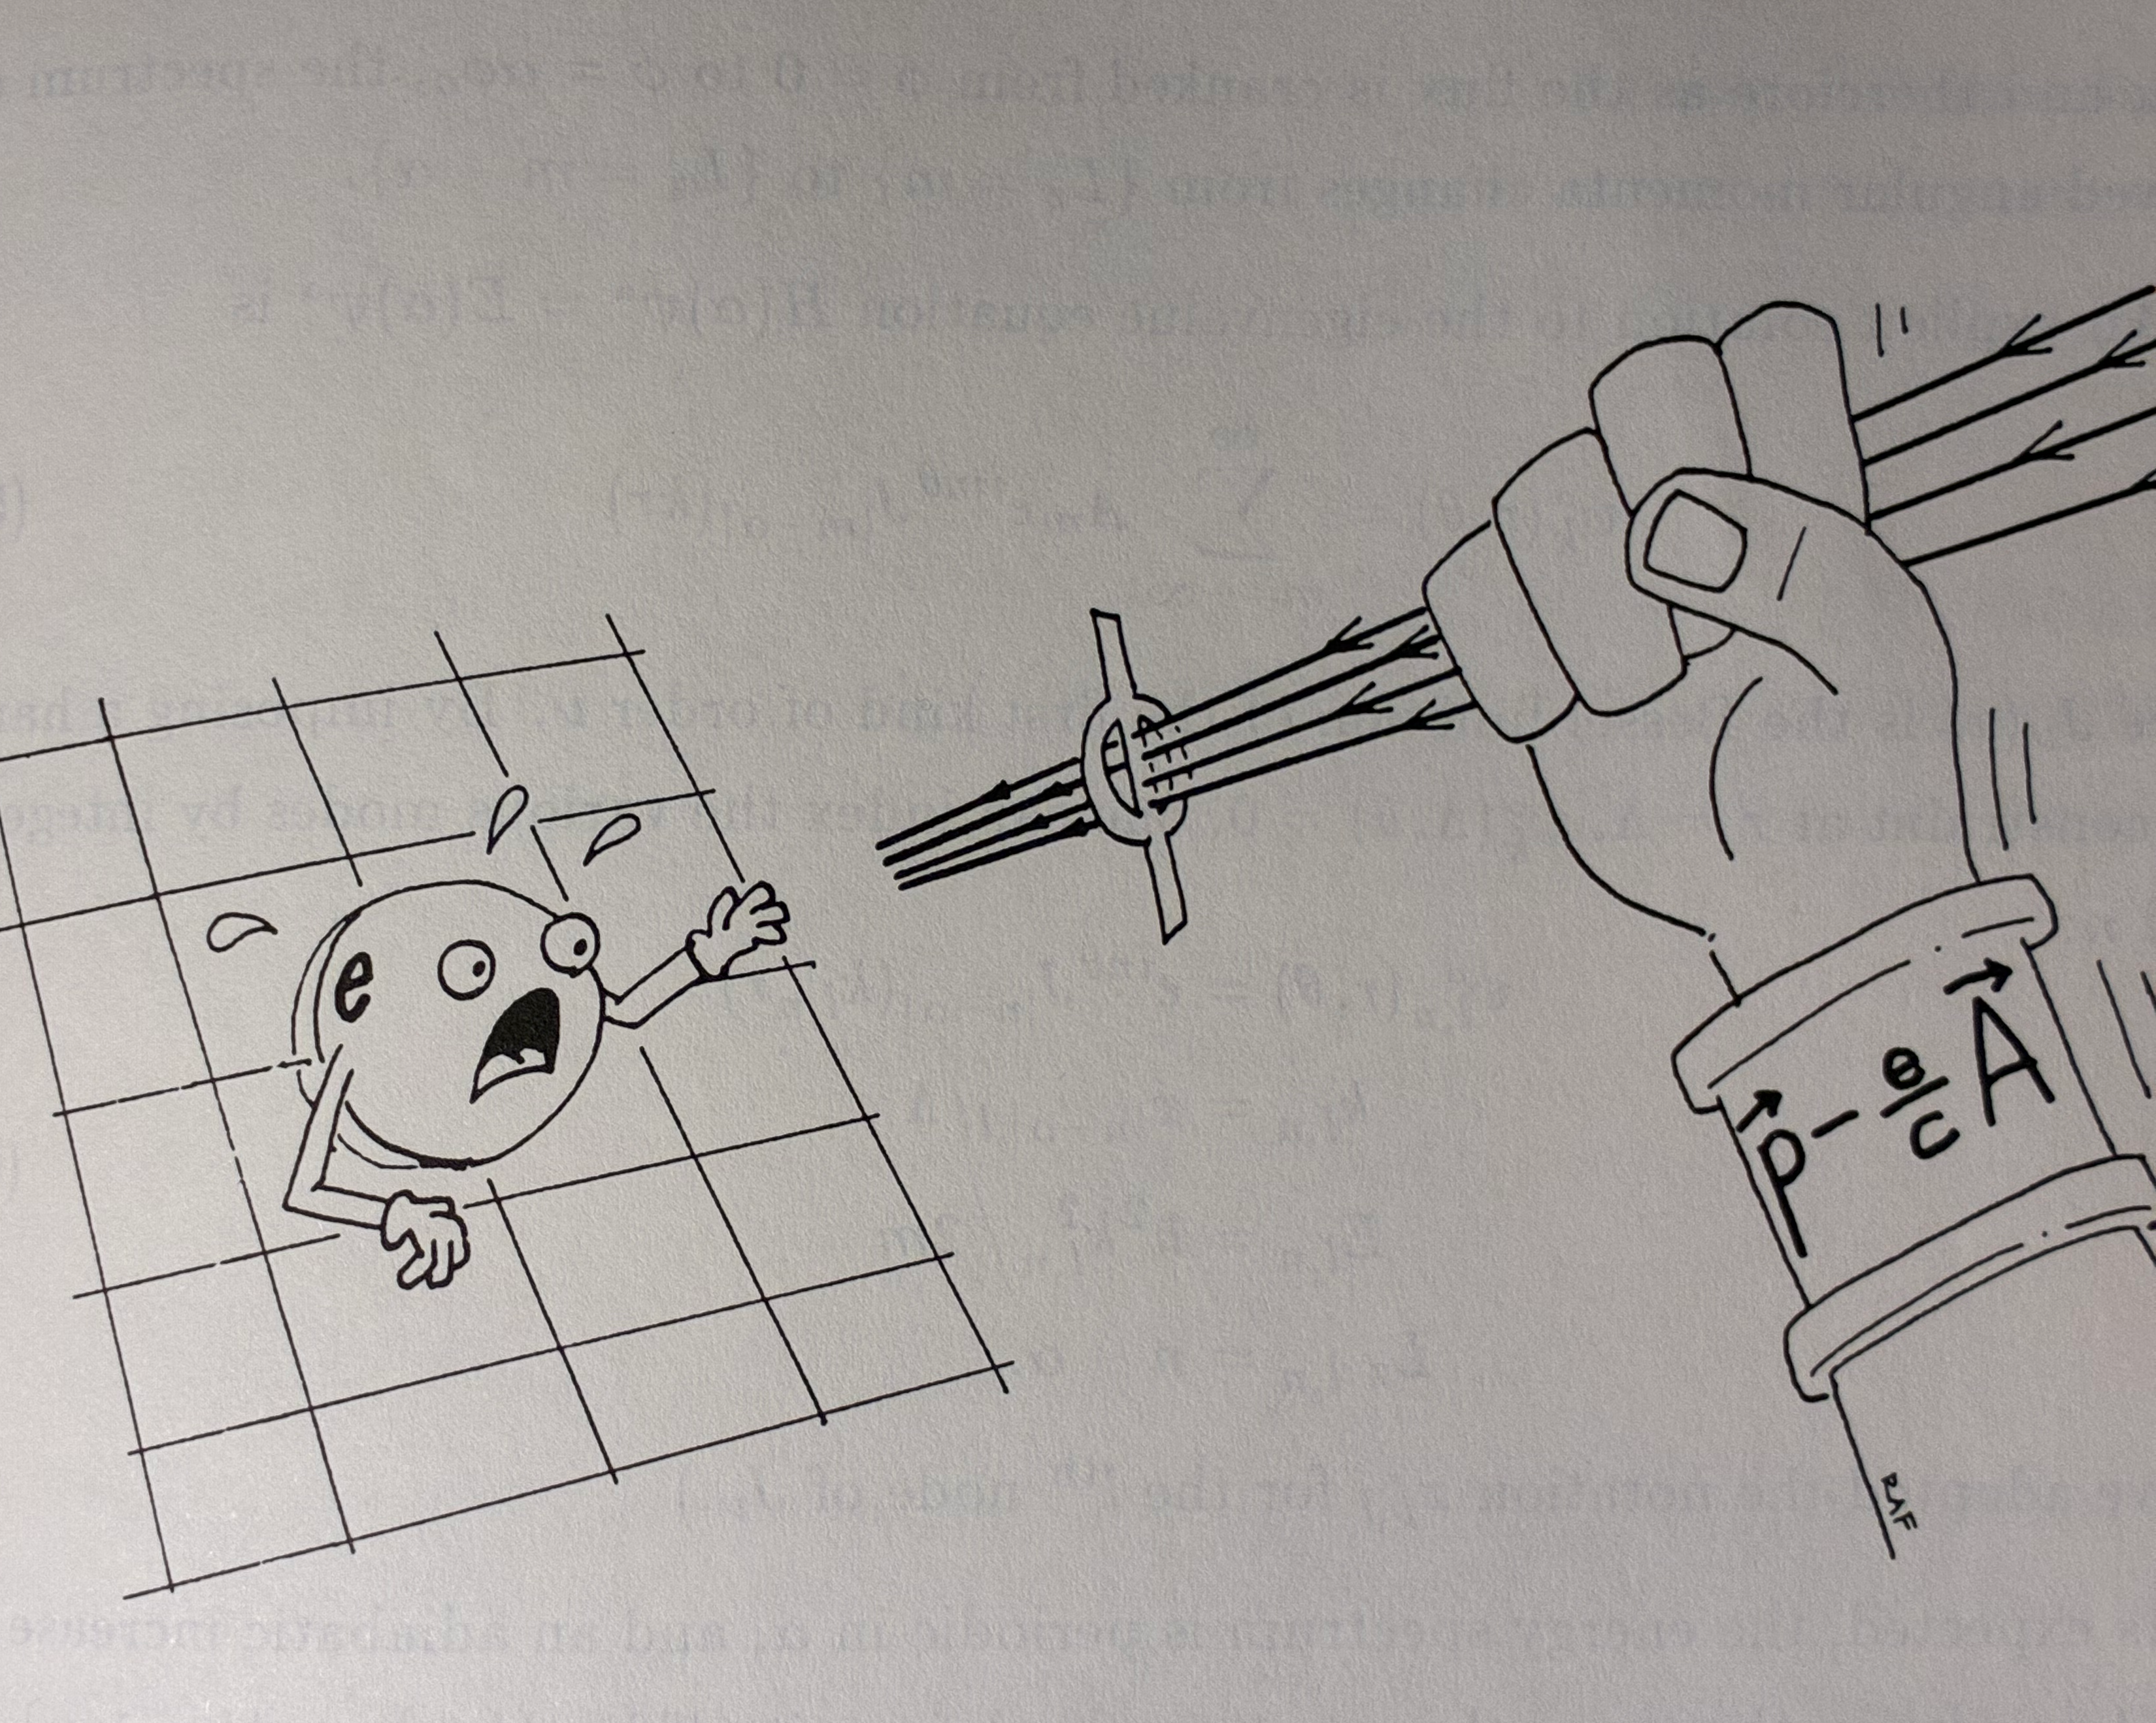
\includegraphics[width=\textwidth]{fluxtube}
  \caption{Illustration of anyon as a particle-flux tube composite. Illustration taken form D.  P. Avoras ”Geometric Phases in Physics”, pg. 287, ed. A. Shapere and F. Wilczek, World Scientific (1989)}
  \label{fluxt}
\end{figure}

We shall assume the latter for the nuclei of our collision partners. Hence, the Hamiltonian for a 2D Hydrogen atom/ion pair, whose nuclei are anyons, takes the form

\begin{equation}
  H =\frac{1}{2 m} \left ({\bf p}_{1} - {\bf A} \right)^2 + \frac{1}{2 m} ({\bf p}_{2} - {\bf A} )^2 + H'({\bf r}_{1},{\bf r}_{2} )
\end{equation}
where $H'({\bf r}_{1},{\bf r}_{2})$ includes the electronic kinetic energy an all Coulombic interactions discussed in the previous chapters and 

\begin{equation}
{\bf A} \equiv  \alpha \, \frac{{\bf n} \times ({\bf r}_{1} - {\bf r}_{2}  ) }{|{\bf r}_{1} -{\bf r}_{2} |^2}
\end{equation}
is a gauge potential \cite{Wu1984PRL53_111}. Here $ {\bf n}$ is a unit normal vector to the 2D scattering plane and $ 0 < \alpha <1. $ Introducing the relative coordinates

\begin{equation}
\begin{split}
& {\bf R}= {\bf r}_{2} -{\bf r}_{1}  \\
& {\bf R}_{cm} = \frac{1}{2} \, ( {\bf r}_{2} + {\bf r}_{1} )
\end{split}
\end{equation}
The Schrodinger equation for the relative motion $F({\bf R})$ becomes
\begin{equation}
 -\frac{1}{2 \mu} ({\bf \nabla} - i \, {\bf A})^2  F({\bf R}) + V_{g,u}(R) F({\bf R}) - E F({\bf R}) =0
\end{equation}
where ${\bf \nabla}$ is  the 2D gradiant operator and, in a cylindrical coordinate system,
\begin{equation}
{\bf A} = {\hat {\bf \phi} } \, \frac{\alpha}{R}
\end{equation}
Or
\begin{equation}
\begin{split}
& \frac{d^2 F({\bf R})}{d R^2} + \frac{ d F({\bf R})}{d R} \frac{1}{R} +\frac{1}{R^2} \left (\frac{\partial}{\partial \phi} - i \, \alpha \right )^2 F({\bf R}) +  \\
& (k^2 -2 \mu V_{g,u}(R)) F({\bf R}) = 0
\end{split}
\end{equation}
Note that if we impose a singular gauge transformation 
$ F({\bf R}) \rightarrow \exp(i \, \alpha \, \phi) {\tilde F}({\bf R}) $ then 
$ {\tilde F}(\bf R) $ obeys the standard Schrodinger without the presence of a flux tube, however, the pre-factor $e^{i \, \alpha }$ introduces multi-valuedness in the total amplitude and special methods \cite{Berry1980_AB_exact} must be invoked to cancel that singularity. Under
particle interchange $ {\bf R} \rightarrow -{\bf R} $, which in this coordinate system is equivalent to the  action of the parity operator ${\bf  \Pi}. $

Here, we follow the procedure of Aharonov-Bohm and expand $F({\bf R}) $ in terms of
single-valued function $ e^{i m \phi} $, $ m=0,\pm1, \dots $, resulting in the
the radial equations \eqref{AhBo2}
\begin{equation}\label{AhBo2}
F_{m}''(R) + \frac{F'_{m}}{R} - \frac{(m- \alpha)^2}{R^2} F_{m}(R) + (k^2 - 2 \mu V_{g,u}(R)) F_{m}(R) =0
\end{equation}
from which we construct the amplitude in the asymptotic region
\begin{equation}\label{AhBo3}
\sum_{m=0,\pm1,...} \exp(i m \phi) \, \left ( a_{m} \, J_{|m-\alpha | }(k R)  + b_{m} {H^{(1)}}_{|m - \alpha |} (k R) \right )
\end{equation}
If we choose (see \eqref{AhBo3}) $ a_{m} = (- i)^{| m - \alpha |}  $,  the above expression reduces to

\begin{equation}\label{ReducedAB}
F_{g,u} \rightarrow \exp(i \alpha \phi) \exp(-i k z) + \frac{\exp(i k R)}{\sqrt{2 \pi k R} } f_{AB}(\phi) + f^{g,u}(\phi) \frac{\exp(i k R)}{\sqrt{ R} }
\end{equation}

where $f_{AB} $ is the Aharonov-Bohm scattering amplitude, and $ f_{g,u}(\phi) $ is given by the expression

\begin{equation}\label{AhBoutWave}
  \begin{split}
& f^{g,u}(\phi) =\sqrt{\frac{2}{\pi k}} \, \sum_{m=0, \pm 1 \dots} {(-i)}^{|m-\alpha |}  \exp(i m \phi) \, b^{g,u}_{m} \\
& b^{g,u}_{m}= {(-i)}^{| m -\alpha | } \frac{J'_{| m-\alpha | }- y^{g,u}_{m} J_{|m -\alpha|} }{ H'_{| m-\alpha |} - y^{g,u}_{m} H_{|m-\alpha|}} 
\end{split}
\end{equation}
and $J', H'$ represent derivatives with respect to R, and $ y^{g,u}$ the log-derivates corresponding to gerade and ungerade potentials respectively Note that the wave amplitude, though single valued, the incident wave in equation \eqref{ReducedAB} is multi-valued.
As Schrodinger equation \eqref{Schr2DAnyon} is invariant to the parity operation $ {\bf \Pi}$, weseek the eigensolutions $F({\bf R})$ that are either even or odd with respect to a parity transformation, i.e.${\bf \Pi}\, F({\bf R}) = F({\bf R}) $ or
${\bf \Pi} \, F({\bf R}) = -F({\bf R}) $ for even/odd functions respectively. We shall call the former the bosonic/fermionic bases respectively.

Following the discussion leading to equation \eqref{ReducedAB} e obtain the outgoing wave
of the charge transfer amplitude given by Eq. \eqref{AhBoutWave} but where
 $ b_{|m|}^{g,u} $ satisfies relation \eqref{AhBoutWave}  instead of \eqref{bm2DReg}, and we get
\begin{equation}
\begin{split}
&\sigma_{CT} = \frac{2}{k} \left (\sum_{m} | b^{(g)}_{m} - b^{(u)}_{m} |^2 \right ) \\
& m=0, \pm 2, \dots \quad {\rm for \, bosonic \, base} \\
& m=\pm 1, \pm 3 \quad {\rm for \, fermionic \, base}
\end{split}
/\end{equation}

Not/
e that the terms proportional to $ f_{AB}(\phi) $ cancel as they are independent of the gerade/ungerade potentials. The restriction to odd values of $ m$ is determined by the fermionic symmetry requirement of the base $(\alpha=0)$ system.  

\section{Calculations and Discussion}
Below we illustrate the result of the calculations corresponding to the analysis given above.

In Figures  2-7 we present values for the calculation of the partial wave contributions to
$ | b^{(g)}_{m} - b^{(u)}_{m} |^2 $ for the values of temperatures from $T=1, 10, 100k \, K. $ The abcissa correspond to the partial wave index $m$, and the blue/red icons refer to bosonic/fermionic basis respectively. The parameter $\alpha$ gives the strength of the flux tube, so $\alpha =0$ corresponds to the absence of a flux tube, and the partial wave contributions reflect the standard symmetry identification for the 3D case.
For $\alpha=1$, the Wilson loop integral
\begin{equation}
\oint_{C} {\bf A}\cdot d{\bf r} = 2 \pi \, n
\end{equation}
where $C$ is any circuit enclosing the flux with winding number $ n.$ In that case we notice, from these figures, that he  partial wave spectra
are identical to the $\alpha=0 $ spectra, with the important difference that the bosonic 
$\alpha =0 $, contributions now correspond to the fermionic $\alpha=1$ contributions, and vice/versa. One can interpret this phenomenon as a transmutation of bosons into fermions, and vice/versa.

The case $\alpha=1/2$ exhibits fractional statistics, and
in order to distinguish it from bosonic/fermionic statistics, particles that exhibit this feature
are commonly called semions
in the literature (cite papers).  In the figures below, we also
illustrate the partial wave contributions for semions $(\alpha=1/2)$, at $ T=1K, 10K, 100K.$

\begin{figure} [H]  
    \centering 
    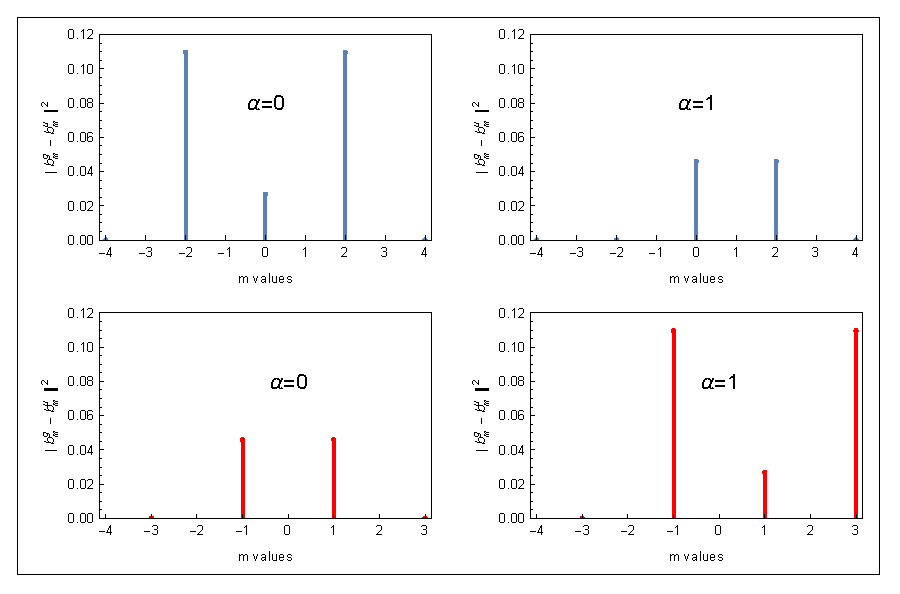
\includegraphics[width = \textwidth]{fig1a.pdf}
    \caption{Collison temperature $T= 1 \, K. $ Blue icons refer to a bosonic base, and red icons to a fermionic base.}
    \label{fig:one} 
\end{figure}

\begin{figure} [H]  
    \centering 
    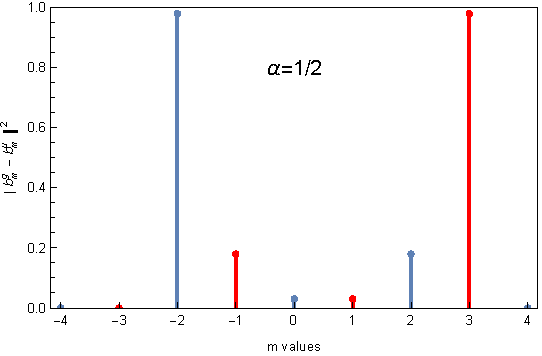
\includegraphics[width = 0.7\textwidth]{fig1b.pdf}
    \caption{Collison temperature $T= 1 \, K. $ Blue icons refer to a bosonic base, and red icons to a fermionic base. }
    \label{fig:one} 
\end{figure}

\begin{figure} [H] 
    \centering 
    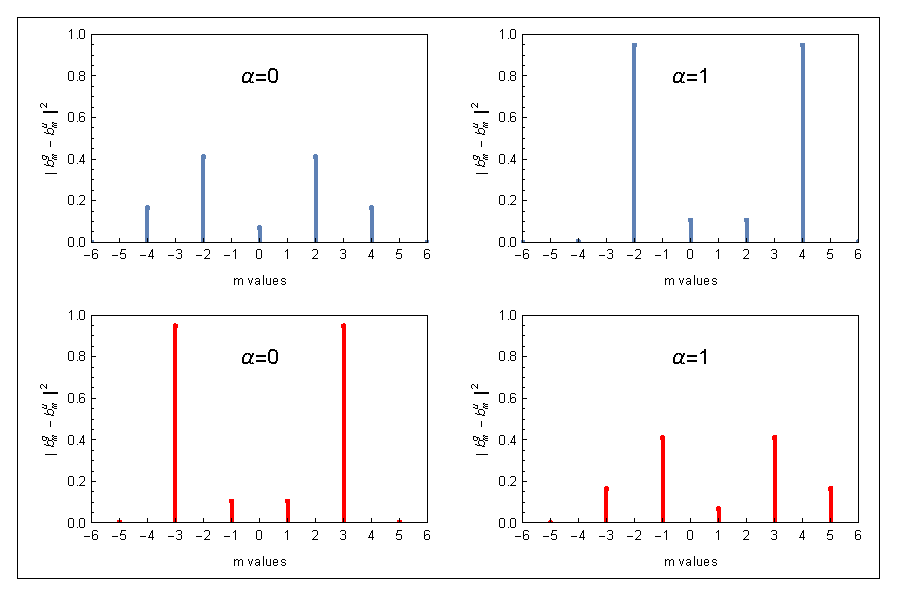
\includegraphics[width = \textwidth]{fig2a.pdf}
    \caption{Collision tempearture $T=10 \, K.$ Blue icons refer to a bosonic base, and red icons to a fermionic base. }
    \label{fig:one} 
\end{figure}

\begin{figure} [H] 
    \centering 
    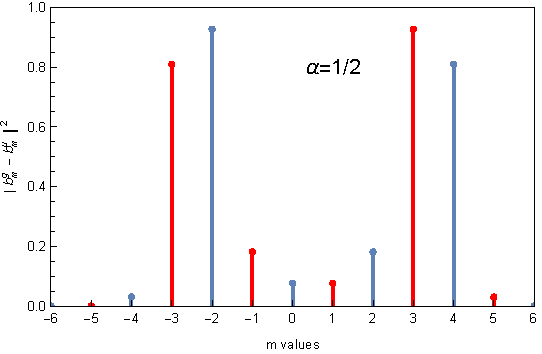
\includegraphics[width = 0.7\textwidth]{fig2b.pdf}
    \caption{Collision temperature $ T=10 \, K. $ Blue icons refer to a bosonic base, and red icons to a fermionic base. }
    \label{fig:one}
\end{figure}


\begin{figure} [H] 
    \centering 
    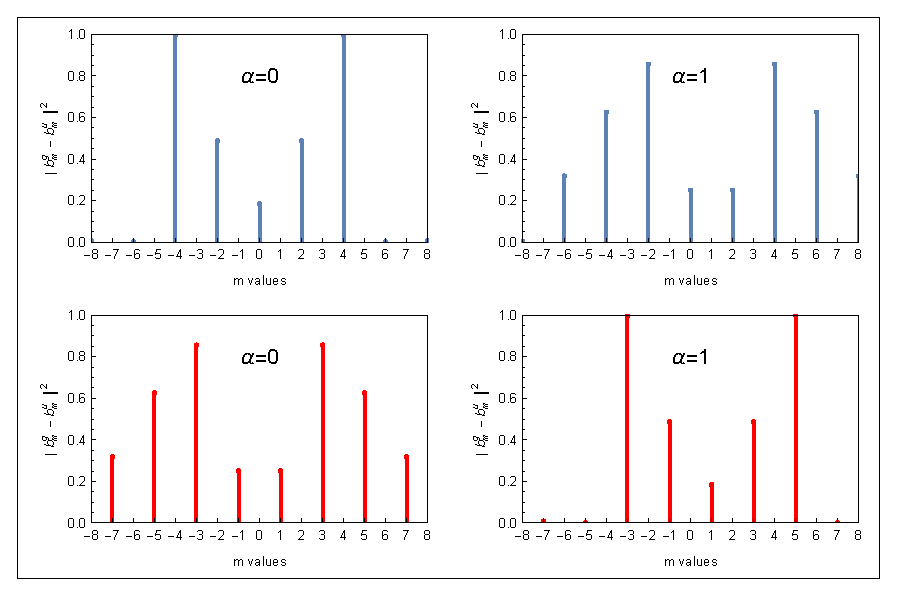
\includegraphics[width = \textwidth]{fig3a.pdf}
    \caption{Collision temperature $T=100 \, K. $ Blue icons refer to a bosonic base, and red icons to a fermionic base. }
    \label{fig:one} 
\end{figure}

\begin{figure} [H] 
    \centering 
    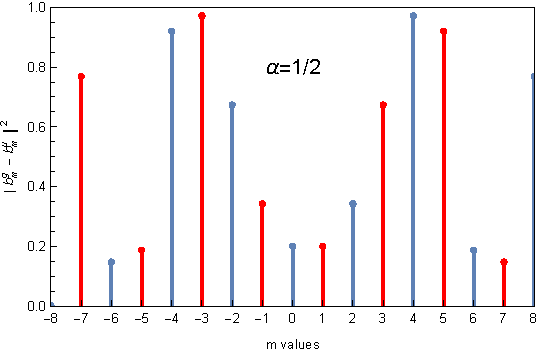
\includegraphics[width = 0.7\textwidth]{fig3b.pdf}
    \caption{Collision temperature $T=100 \, K. $ Blue icons refer to a bosonic base, and red icons to a fermionic base. Flux tube charge $\alpha=0$, and $T=1 K $}
    \label{fig:one} 
\end{figure}


\begin{figure} [H] 
    \centering 
    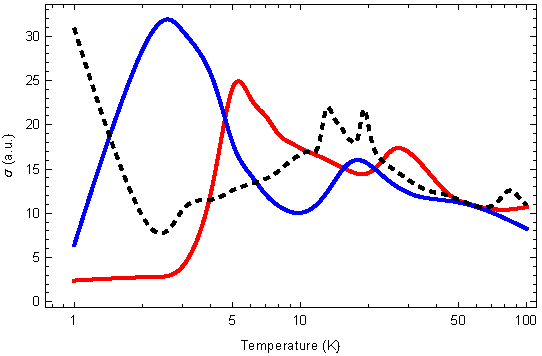
\includegraphics[width = 0.9\textwidth]{CT.pdf}
    \caption{Total RCT cross sections. Solid lines refer to $ \alpha=0$ (i.e., absence of flux tube), for the bosonic base (Blue line) and the fermionic base (Red line) respectively. The dashed line refers to a semion $(\alpha=1/2)$, and the cross section is identical for both fermionic and bosonic bases.}
     \label{fig:one} % this internally labels the figure for future referencing.
\end{figure}



